% Seminarul 0: Introducere: componente și netezire exponențială
% Serii de timp -- Programele de licență Informatică economică și Cibernetică economică, Academia de Studii Economice din București
% GENERAT de latex/build_seminar0.py -- modificați generatorul, nu acest fișier.
% Implicit versiunea pentru studenți; versiunea profesorului este wrapper-ul *_solutions.tex.
\makeatletter\@ifundefined{ifsolutions}{\expandafter\newif\csname ifsolutions\endcsname}{}\makeatother

\newcommand{\coursename}{Serii de timp}
\def\tsalang{ro}
% Preambul comun TSA -- Serii de timp / Time Series Analysis (Beamer, 16:9)
% Același design ca MFM și SFM (preluat din SFM, 5 octombrie 2026). Înainte de % Preambul comun TSA -- Serii de timp / Time Series Analysis (Beamer, 16:9)
% Același design ca MFM și SFM (preluat din SFM, 5 octombrie 2026). Înainte de % Preambul comun TSA -- Serii de timp / Time Series Analysis (Beamer, 16:9)
% Același design ca MFM și SFM (preluat din SFM, 5 octombrie 2026). Înainte de \input{../../latex/preamble} se definește
%   \newcommand{\coursename}{Time Series Analysis}      (EN)
%   \newcommand{\coursename}{Serii de timp}       (RO)  și  \def\tsalang{ro}
% Fișierele .tex se află în EN/Courses, EN/Seminars, RO/Cursuri, RO/Seminarii (două niveluri sub rădăcină).
% Deck-urile sînt generate de latex/build_chapterN.py / build_seminarN.py (vezi latex/tsa_build.py).

\documentclass[9pt, aspectratio=169, t]{beamer}
\providecommand{\coursename}{Time Series Analysis}

% Ensure content fits on slides
\setbeamersize{text margin left=8mm, text margin right=8mm}
% Smaller institute font (title page)
\setbeamerfont{institute}{size=\footnotesize}

%=============================================================================
% THEME AND STYLE CONFIGURATION
%=============================================================================
\usetheme{default}
% Using default theme for clean header/footer control

% Color Palette (matching Redispatch PDF)
\definecolor{MainBlue}{RGB}{26, 58, 110}
\definecolor{AccentBlue}{RGB}{26, 58, 110}
\definecolor{IDAred}{RGB}{205, 0, 0}
\definecolor{DarkGray}{RGB}{51, 51, 51}
\definecolor{MediumGray}{RGB}{128, 128, 128}
\definecolor{LightGray}{RGB}{248, 248, 248}
\definecolor{VeryLightGray}{RGB}{235, 235, 235}
\definecolor{KeynoteGray}{RGB}{218, 218, 218}
\definecolor{SectionGray}{RGB}{120, 120, 120}
\definecolor{FooterGray}{RGB}{100, 100, 100}
\definecolor{Crimson}{RGB}{220, 53, 69}
\definecolor{Forest}{RGB}{46, 125, 50}
\definecolor{Amber}{RGB}{181, 133, 63}
\definecolor{Orange}{RGB}{230, 126, 34}
\definecolor{Purple}{RGB}{142, 68, 173}

% Gradient background (exact Keynote 315° gradient: white to RGB 218,218,218)
\setbeamertemplate{background}{%
    \begin{tikzpicture}[remember picture, overlay]
        \shade[shading=axis, shading angle=315,
        top color=white, bottom color=KeynoteGray]
        (current page.south west) rectangle (current page.north east);
    \end{tikzpicture}%
}
% Fallback solid color for compatibility
\setbeamercolor{background canvas}{bg=}

\setbeamercolor{palette primary}{bg=MainBlue, fg=white}
\setbeamercolor{palette secondary}{bg=MainBlue!85, fg=white}
\setbeamercolor{palette tertiary}{bg=MainBlue!70, fg=white}
\setbeamercolor{structure}{fg=MainBlue}
\setbeamercolor{title}{fg=IDAred}
\setbeamercolor{frametitle}{fg=IDAred, bg=}
\setbeamercolor{block title}{bg=MainBlue, fg=white}
\setbeamercolor{block body}{bg=VeryLightGray, fg=DarkGray}
\setbeamercolor{block title alerted}{bg=Crimson, fg=white}
\setbeamercolor{block body alerted}{bg=Crimson!8, fg=DarkGray}
\setbeamercolor{block title example}{bg=Forest, fg=white}
\setbeamercolor{block body example}{bg=Forest!8, fg=DarkGray}
\setbeamercolor{item}{fg=MainBlue}

% Footer colors (override Madrid theme blue)
\setbeamercolor{author in head/foot}{fg=FooterGray, bg=}
\setbeamercolor{title in head/foot}{fg=FooterGray, bg=}
\setbeamercolor{date in head/foot}{fg=FooterGray, bg=}
\setbeamercolor{section in head/foot}{fg=FooterGray, bg=}
\setbeamercolor{subsection in head/foot}{fg=FooterGray, bg=}

% Bullet styles (apply everywhere including blocks)
\setbeamertemplate{itemize item}{\color{MainBlue}$\boxdot$}
\setbeamertemplate{itemize subitem}{\color{MainBlue}$\blacktriangleright$}
\setbeamertemplate{itemize subsubitem}{\color{MainBlue}\tiny$\bullet$}
\setbeamertemplate{itemize/enumerate body begin}{\normalsize}
\setbeamertemplate{itemize/enumerate subbody begin}{\normalsize}

% Item spacing - compact style
\setlength{\leftmargini}{10pt}       % Level 1: minimal indent
\setlength{\leftmarginii}{10pt}      % Level 2: minimal additional indent
% Compact list spacing (zero extra space before/after lists in blocks)
\makeatletter
\def\@listi{\leftmargin\leftmargini \topsep 0pt \parsep 0pt \itemsep 0pt}
\def\@listii{\leftmargin\leftmarginii \topsep 0pt \parsep 0pt \itemsep 0pt}
\makeatother

\setbeamertemplate{navigation symbols}{}

%=============================================================================
% CUSTOM HEADLINE
%=============================================================================
\setbeamertemplate{headline}{%
    \vskip10pt%
    \hbox to \paperwidth{%
        \hskip0.5cm%
        {\small\color{FooterGray}\renewcommand{\hyperlink}[2]{##2}\insertsectionhead}%
        \hfill%
        \textcolor{FooterGray}{\small\insertframenumber}%
        \hskip0.5cm%
    }%
    \vskip4pt%
    {\color{FooterGray}\hrule height 0.4pt}%
}

%=============================================================================
% CUSTOM FOOTER
%=============================================================================
\usepackage{fontawesome5}

\setbeamertemplate{footline}{%
    {\color{FooterGray}\hrule height 0.4pt}%
    \vskip4pt%
    \hbox to \paperwidth{%
        \hskip0.5cm%
        \textcolor{FooterGray}{\small\coursename}%
        \hfill%
        \raisebox{-0.1em}{%
            \begin{tikzpicture}[x=0.08em, y=0.08em, line width=0.4pt]
                \draw[FooterGray] (0,3) -- (1,4) -- (2,3.5) -- (3,5) -- (4,4) -- (5,6) -- (6,5.5) -- (7,4) -- (8,5) -- (9,7) -- (10,6) -- (11,5) -- (12,6.5) -- (13,8) -- (14,7) -- (15,6) -- (16,7.5) -- (17,9) -- (18,8) -- (19,7) -- (20,8.5) -- (21,10) -- (22,9) -- (23,8) -- (24,9.5);
            \end{tikzpicture}%
        }%
        \hskip0.5cm%
    }%
    \vskip6pt%
}

%=============================================================================
% PACKAGES
%=============================================================================
\usepackage[utf8]{inputenc}
\DeclareUnicodeCharacter{03B1}{\ensuremath{\alpha}}
\usepackage[T1]{fontenc}
\usepackage{amsmath, amssymb, amsthm}
\usepackage{mathtools}
\usepackage{bm}
\usepackage{tikz}
\usetikzlibrary{arrows.meta, positioning, shapes, calc, decorations.pathreplacing, shadings}
\usepackage{booktabs}
\usepackage{multirow}
\usepackage{array}
\usepackage{graphicx}
\usepackage{animate}
\usepackage{hyperref}
\usepackage{colortbl}
\usepackage{listings}
\lstset{language=Python, basicstyle=\ttfamily\scriptsize, keywordstyle=\color{MainBlue}\bfseries,
  commentstyle=\color{Forest}, stringstyle=\color{Crimson}, breaklines=true,
  frame=none, backgroundcolor=\color{VeryLightGray}, xleftmargin=2mm}
\hypersetup{colorlinks=true, linkcolor=MainBlue, urlcolor=MainBlue}
\graphicspath{{../../logos/}{../../charts/}{../../photos/}}
\usepackage{xcolor}
\hfuzz=2pt  % Suppress tiny overfull warnings (<2pt)
\vfuzz=2pt  % Suppress tiny vertical overfull warnings (<2pt)
% \mathrm in the sans-serif family of the slides (beamer resets \mathrm to the serif family at \begin{document};
% this hook runs after beamer's, so WN, Var, RMSE, ... in formulas match the surrounding text)
% Bold vectors and matrices in the same sans-serif family: \mathbf{A} in sans bold (beamer's own \mathbf came out in
% medium weight), and the bold upright Greek capitals of \boldsymbol / \bm (\bSigma, \bPhi, \boldsymbol{\Theta}) in
% cmss bold: bm.sty fixes its "boldoperators" font when it is loaded (serif cmbx), before beamer switches the
% operators to cmss, so it is reset here.
\AtBeginDocument{%
  \SetMathAlphabet{\mathrm}{normal}{\encodingdefault}{\sfdefault}{\mddefault}{n}%
  \SetMathAlphabet{\mathrm}{bold}{\encodingdefault}{\sfdefault}{bx}{n}%
  \SetMathAlphabet{\mathbf}{normal}{\encodingdefault}{\sfdefault}{bx}{n}%
  \SetMathAlphabet{\mathbf}{bold}{\encodingdefault}{\sfdefault}{bx}{n}%
  \SetSymbolFont{boldoperators}{normal}{OT1}{cmss}{bx}{n}%
  \SetSymbolFont{boldoperators}{bold}{OT1}{cmss}{bx}{n}}

%=============================================================================
% QUANTLET COMMANDS
%   \quantlet{<displayed name>}{<url>}       (generic, compatible with the older TSA decks)
%   \tsaquantlet{Ch_05}{TSA_ch5_garch}       -> https://github.com/danpele/Time-Series-Analysis/tree/main/Quantlets/Ch_05/TSA_ch5_garch
%   \qlurl{<folder>} is defined per chapter by the generator (Quantlets/Ch_NN/<folder>)
%=============================================================================
\newcommand{\tsarepo}{https://github.com/danpele/Time-Series-Analysis}
\newcommand{\tsaqlbase}{https://github.com/danpele/Time-Series-Analysis/tree/main/Quantlets}
\newcommand{\quantlet}[2]{%
    \hfill\href{#2}{%
        \raisebox{-0.15em}{
\includegraphics[height=0.7em]{ql_logo.png}}%
        \textcolor{MainBlue}{\tiny\ #1}%
    }%
}
\newcommand{\tsaquantlet}[2]{\quantlet{\detokenize{#2}}{\tsaqlbase/#1/#2}}

%=============================================================================
% NOTEBOOKS (Google Colab)
%   \colaburl{notebooks/EN/chapter5_seminar_notebook.ipynb} -> the Colab link of a file in the TSA repo
%   \nb: the chapter notebook (each seminar deck redefines it with \renewcommand)
%=============================================================================
\newcommand{\colaburl}[1]{https://colab.research.google.com/github/danpele/Time-Series-Analysis/blob/main/#1}
\newcommand{\nb}{https://colab.research.google.com/github/danpele/Time-Series-Analysis/tree/main/notebooks/EN}
\newcommand{\nbname}{notebooks/EN}

%=============================================================================
% SLIDE HELPERS (used by the generators; the same as in MFM)
%=============================================================================
% local font size for list bodies (the preamble forces \normalsize)
\newcommand{\itemsize}[1]{\setbeamertemplate{itemize/enumerate body begin}{#1}\setbeamertemplate{itemize/enumerate subbody begin}{#1}}
\newcommand{\intitle}[1]{{\hypersetup{urlcolor=white}#1}}   % white links inside coloured title bars
\newcommand{\imgcap}[1]{{\scriptsize #1}\\[0.5mm]}          % caption under a photo
\newcommand{\imgcredit}[2]{{\tiny\color{FooterGray}\href{#1}{#2}}}   % image credit: source URL, author/licence
\newcommand{\aiprompt}[1]{{\ttfamily\color{MainBlue}#1}}     % a prompt to an AI assistant

%=============================================================================
% SEMINARS: student version by default; the instructor wrapper *_solutions.tex sets \solutionstrue
%=============================================================================
\makeatletter\@ifundefined{ifsolutions}{\expandafter\newif\csname ifsolutions\endcsname}{}\makeatother
\newcommand{\solonly}[1]{\ifsolutions #1\fi}
\newcommand{\propsub}{\ifsolutions\else\framesubtitle{\ifdefined\tsalang Rezolvarea se discută la seminar\else Solution discussed in class\fi}\fi}

%=============================================================================
% APPENDIX AND CHAPTER LINKS (latex/appendix_links.py writes the calls; it also re-declares these
% macros before \begin{document}, so the decks compile with or without this preamble block)
%=============================================================================
\providecommand{\tsaapplink}[3]{\hypertarget{#2}{}\hyperlink{#1}{\beamergotobutton{#3}}}
\providecommand{\tsaappback}[2]{\begin{tikzpicture}[remember picture,overlay]\node[anchor=south east] at ([xshift=-3mm,yshift=7mm]current page.south east){\hyperlink{#1}{\beamerreturnbutton{#2}}};\end{tikzpicture}}
\providecommand{\tsachlink}[2]{\href{#1}{#2}}
\providecommand{\tsachlinkt}[2]{\href{#1}{\usebeamercolor[fg]{frametitle}#2}}

%=============================================================================
% QUANTINAR COMMAND: link către un curs Quantinar (subiecte avansate)
%=============================================================================
\newcommand{\quantinar}[2]{%
    \href{#2}{%
        \raisebox{-0.15em}{
\includegraphics[height=0.8em]{qr_logo.png}}%
        \textcolor{MainBlue}{\scriptsize\ #1}%
    }%
}

%=============================================================================
% CUSTOM TITLE PAGE
%=============================================================================
\defbeamertemplate*{title page}{hybrid}[1][]
{
    \vspace{0.2cm}
    % Logos row - top header (with clickable links)
    \begin{center}
        \href{https://www.ase.ro}{
\includegraphics[height=1.0cm]{ase_logo.png}}\hspace{0.3cm}%
        \href{https://theida.net}{
\includegraphics[height=1.0cm]{ida_logo.png}}\hspace{0.3cm}%
        \href{https://blockchain-research-center.com}{
\includegraphics[height=1.0cm]{brc_logo.png}}\hspace{0.3cm}%
        \href{https://www.ai4efin.ase.ro}{
\includegraphics[height=1.0cm]{ai4efin_logo.png}}\hspace{0.3cm}%
        \href{https://ipe.ro/new}{
\includegraphics[height=1.0cm]{acad_logo.png}}\hspace{0.3cm}%
        \href{https://www.digital-finance-msca.com}{
\includegraphics[height=1.0cm]{msca_logo.png}}%
    \end{center}

    \vspace{0.6cm}

    % Main title with Q logos on sides (with clickable links)
    \begin{center}
        \begin{minipage}{0.1\textwidth}
            \centering
            \href{https://quantlet.com}{
\includegraphics[height=1.1cm]{ql_logo.png}}
        \end{minipage}%
        \begin{minipage}{0.78\textwidth}
            \centering
            {\LARGE\bfseries\usebeamercolor[fg]{title}\inserttitle}

            \vspace{0.3cm}

            {\usebeamerfont{subtitle}\usebeamercolor[fg]{title}\insertsubtitle}
        \end{minipage}%
        \begin{minipage}{0.1\textwidth}
            \centering
            \href{https://quantinar.com}{
\includegraphics[height=1.1cm]{qr_logo.png}}
        \end{minipage}
    \end{center}

    \vspace{0.6cm}

    % Authors (left aligned)
    \hspace{0.5cm}{\usebeamerfont{author}\insertauthor}

    \vspace{0.3cm}

    % Institute/Affiliations (left aligned)
    \hspace{0.5cm}\begin{minipage}[t]{0.9\textwidth}
        \raggedright\small\insertinstitute
    \end{minipage}
}

%=============================================================================
% THEOREM ENVIRONMENTS
%=============================================================================
\theoremstyle{definition}
\setbeamertemplate{theorems}[numbered]
\ifdefined\tsalang
\newtheorem{defn}{Definiție}
\newtheorem{thm}{Teoremă}
\newtheorem{prop}{Propoziție}
\newtheorem{rmk}{Observație}
\else
\newtheorem{defn}{Definition}
\newtheorem{thm}{Theorem}
\newtheorem{prop}{Proposition}
\newtheorem{rmk}{Remark}
\fi

%=============================================================================
% CENTRED MINIPAGE (no extra vertical space)
%=============================================================================
\newenvironment{cminipage}[1]{%
    \par\noindent\hfill\begin{minipage}{#1}\ignorespaces
}{%
    \end{minipage}\hfill\null\par
}

%=============================================================================
% CUSTOM COMMANDS
%=============================================================================
\newcommand{\E}{\mathbb{E}}
\newcommand{\Var}{\text{Var}}
\newcommand{\Cov}{\text{Cov}}
\newcommand{\Corr}{\text{Corr}}
\newcommand{\R}{\mathbb{R}}
\newcommand{\N}{\mathbb{N}}
\newcommand{\Z}{\mathbb{Z}}
\newcommand{\B}{\mathbf{B}}
\newcommand{\imark}{\textcolor{MainBlue}{\textbullet}}
\newcommand{\RMSE}{\text{RMSE}}
\newcommand{\MAE}{\text{MAE}}
\newcommand{\MAPE}{\text{MAPE}}

% Boldface vector/matrix commands (VAR, VECM, state space; also used by the older TSA decks)
\newcommand{\bY}{\mathbf{Y}}
\newcommand{\bX}{\mathbf{X}}
\newcommand{\bA}{\mathbf{A}}
\newcommand{\bB}{\mathbf{B}}
\newcommand{\bepsilon}{\boldsymbol{\varepsilon}}
\newcommand{\bSigma}{\boldsymbol{\Sigma}}
\newcommand{\bPhi}{\boldsymbol{\Phi}}
\newcommand{\bGamma}{\boldsymbol{\Gamma}}
\newcommand{\bPi}{\boldsymbol{\Pi}}
\newcommand{\bc}{\mathbf{c}}
\newcommand{\balpha}{\boldsymbol{\alpha}}
\newcommand{\bbeta}{\boldsymbol{\beta}}
\newcommand{\bvarepsilon}{\boldsymbol{\varepsilon}}

% Legacy seminar marks (older TSA seminar decks)
\newcommand{\correct}{\textcolor{Forest}{\checkmark}}
\newcommand{\incorrect}{\textcolor{Crimson}{\texttimes}}
 se definește
%   \newcommand{\coursename}{Time Series Analysis}      (EN)
%   \newcommand{\coursename}{Serii de timp}       (RO)  și  \def\tsalang{ro}
% Fișierele .tex se află în EN/Courses, EN/Seminars, RO/Cursuri, RO/Seminarii (două niveluri sub rădăcină).
% Deck-urile sînt generate de latex/build_chapterN.py / build_seminarN.py (vezi latex/tsa_build.py).

\documentclass[9pt, aspectratio=169, t]{beamer}
\providecommand{\coursename}{Time Series Analysis}

% Ensure content fits on slides
\setbeamersize{text margin left=8mm, text margin right=8mm}
% Smaller institute font (title page)
\setbeamerfont{institute}{size=\footnotesize}

%=============================================================================
% THEME AND STYLE CONFIGURATION
%=============================================================================
\usetheme{default}
% Using default theme for clean header/footer control

% Color Palette (matching Redispatch PDF)
\definecolor{MainBlue}{RGB}{26, 58, 110}
\definecolor{AccentBlue}{RGB}{26, 58, 110}
\definecolor{IDAred}{RGB}{205, 0, 0}
\definecolor{DarkGray}{RGB}{51, 51, 51}
\definecolor{MediumGray}{RGB}{128, 128, 128}
\definecolor{LightGray}{RGB}{248, 248, 248}
\definecolor{VeryLightGray}{RGB}{235, 235, 235}
\definecolor{KeynoteGray}{RGB}{218, 218, 218}
\definecolor{SectionGray}{RGB}{120, 120, 120}
\definecolor{FooterGray}{RGB}{100, 100, 100}
\definecolor{Crimson}{RGB}{220, 53, 69}
\definecolor{Forest}{RGB}{46, 125, 50}
\definecolor{Amber}{RGB}{181, 133, 63}
\definecolor{Orange}{RGB}{230, 126, 34}
\definecolor{Purple}{RGB}{142, 68, 173}

% Gradient background (exact Keynote 315° gradient: white to RGB 218,218,218)
\setbeamertemplate{background}{%
    \begin{tikzpicture}[remember picture, overlay]
        \shade[shading=axis, shading angle=315,
        top color=white, bottom color=KeynoteGray]
        (current page.south west) rectangle (current page.north east);
    \end{tikzpicture}%
}
% Fallback solid color for compatibility
\setbeamercolor{background canvas}{bg=}

\setbeamercolor{palette primary}{bg=MainBlue, fg=white}
\setbeamercolor{palette secondary}{bg=MainBlue!85, fg=white}
\setbeamercolor{palette tertiary}{bg=MainBlue!70, fg=white}
\setbeamercolor{structure}{fg=MainBlue}
\setbeamercolor{title}{fg=IDAred}
\setbeamercolor{frametitle}{fg=IDAred, bg=}
\setbeamercolor{block title}{bg=MainBlue, fg=white}
\setbeamercolor{block body}{bg=VeryLightGray, fg=DarkGray}
\setbeamercolor{block title alerted}{bg=Crimson, fg=white}
\setbeamercolor{block body alerted}{bg=Crimson!8, fg=DarkGray}
\setbeamercolor{block title example}{bg=Forest, fg=white}
\setbeamercolor{block body example}{bg=Forest!8, fg=DarkGray}
\setbeamercolor{item}{fg=MainBlue}

% Footer colors (override Madrid theme blue)
\setbeamercolor{author in head/foot}{fg=FooterGray, bg=}
\setbeamercolor{title in head/foot}{fg=FooterGray, bg=}
\setbeamercolor{date in head/foot}{fg=FooterGray, bg=}
\setbeamercolor{section in head/foot}{fg=FooterGray, bg=}
\setbeamercolor{subsection in head/foot}{fg=FooterGray, bg=}

% Bullet styles (apply everywhere including blocks)
\setbeamertemplate{itemize item}{\color{MainBlue}$\boxdot$}
\setbeamertemplate{itemize subitem}{\color{MainBlue}$\blacktriangleright$}
\setbeamertemplate{itemize subsubitem}{\color{MainBlue}\tiny$\bullet$}
\setbeamertemplate{itemize/enumerate body begin}{\normalsize}
\setbeamertemplate{itemize/enumerate subbody begin}{\normalsize}

% Item spacing - compact style
\setlength{\leftmargini}{10pt}       % Level 1: minimal indent
\setlength{\leftmarginii}{10pt}      % Level 2: minimal additional indent
% Compact list spacing (zero extra space before/after lists in blocks)
\makeatletter
\def\@listi{\leftmargin\leftmargini \topsep 0pt \parsep 0pt \itemsep 0pt}
\def\@listii{\leftmargin\leftmarginii \topsep 0pt \parsep 0pt \itemsep 0pt}
\makeatother

\setbeamertemplate{navigation symbols}{}

%=============================================================================
% CUSTOM HEADLINE
%=============================================================================
\setbeamertemplate{headline}{%
    \vskip10pt%
    \hbox to \paperwidth{%
        \hskip0.5cm%
        {\small\color{FooterGray}\renewcommand{\hyperlink}[2]{##2}\insertsectionhead}%
        \hfill%
        \textcolor{FooterGray}{\small\insertframenumber}%
        \hskip0.5cm%
    }%
    \vskip4pt%
    {\color{FooterGray}\hrule height 0.4pt}%
}

%=============================================================================
% CUSTOM FOOTER
%=============================================================================
\usepackage{fontawesome5}

\setbeamertemplate{footline}{%
    {\color{FooterGray}\hrule height 0.4pt}%
    \vskip4pt%
    \hbox to \paperwidth{%
        \hskip0.5cm%
        \textcolor{FooterGray}{\small\coursename}%
        \hfill%
        \raisebox{-0.1em}{%
            \begin{tikzpicture}[x=0.08em, y=0.08em, line width=0.4pt]
                \draw[FooterGray] (0,3) -- (1,4) -- (2,3.5) -- (3,5) -- (4,4) -- (5,6) -- (6,5.5) -- (7,4) -- (8,5) -- (9,7) -- (10,6) -- (11,5) -- (12,6.5) -- (13,8) -- (14,7) -- (15,6) -- (16,7.5) -- (17,9) -- (18,8) -- (19,7) -- (20,8.5) -- (21,10) -- (22,9) -- (23,8) -- (24,9.5);
            \end{tikzpicture}%
        }%
        \hskip0.5cm%
    }%
    \vskip6pt%
}

%=============================================================================
% PACKAGES
%=============================================================================
\usepackage[utf8]{inputenc}
\DeclareUnicodeCharacter{03B1}{\ensuremath{\alpha}}
\usepackage[T1]{fontenc}
\usepackage{amsmath, amssymb, amsthm}
\usepackage{mathtools}
\usepackage{bm}
\usepackage{tikz}
\usetikzlibrary{arrows.meta, positioning, shapes, calc, decorations.pathreplacing, shadings}
\usepackage{booktabs}
\usepackage{multirow}
\usepackage{array}
\usepackage{graphicx}
\usepackage{animate}
\usepackage{hyperref}
\usepackage{colortbl}
\usepackage{listings}
\lstset{language=Python, basicstyle=\ttfamily\scriptsize, keywordstyle=\color{MainBlue}\bfseries,
  commentstyle=\color{Forest}, stringstyle=\color{Crimson}, breaklines=true,
  frame=none, backgroundcolor=\color{VeryLightGray}, xleftmargin=2mm}
\hypersetup{colorlinks=true, linkcolor=MainBlue, urlcolor=MainBlue}
\graphicspath{{../../logos/}{../../charts/}{../../photos/}}
\usepackage{xcolor}
\hfuzz=2pt  % Suppress tiny overfull warnings (<2pt)
\vfuzz=2pt  % Suppress tiny vertical overfull warnings (<2pt)
% \mathrm in the sans-serif family of the slides (beamer resets \mathrm to the serif family at \begin{document};
% this hook runs after beamer's, so WN, Var, RMSE, ... in formulas match the surrounding text)
% Bold vectors and matrices in the same sans-serif family: \mathbf{A} in sans bold (beamer's own \mathbf came out in
% medium weight), and the bold upright Greek capitals of \boldsymbol / \bm (\bSigma, \bPhi, \boldsymbol{\Theta}) in
% cmss bold: bm.sty fixes its "boldoperators" font when it is loaded (serif cmbx), before beamer switches the
% operators to cmss, so it is reset here.
\AtBeginDocument{%
  \SetMathAlphabet{\mathrm}{normal}{\encodingdefault}{\sfdefault}{\mddefault}{n}%
  \SetMathAlphabet{\mathrm}{bold}{\encodingdefault}{\sfdefault}{bx}{n}%
  \SetMathAlphabet{\mathbf}{normal}{\encodingdefault}{\sfdefault}{bx}{n}%
  \SetMathAlphabet{\mathbf}{bold}{\encodingdefault}{\sfdefault}{bx}{n}%
  \SetSymbolFont{boldoperators}{normal}{OT1}{cmss}{bx}{n}%
  \SetSymbolFont{boldoperators}{bold}{OT1}{cmss}{bx}{n}}

%=============================================================================
% QUANTLET COMMANDS
%   \quantlet{<displayed name>}{<url>}       (generic, compatible with the older TSA decks)
%   \tsaquantlet{Ch_05}{TSA_ch5_garch}       -> https://github.com/danpele/Time-Series-Analysis/tree/main/Quantlets/Ch_05/TSA_ch5_garch
%   \qlurl{<folder>} is defined per chapter by the generator (Quantlets/Ch_NN/<folder>)
%=============================================================================
\newcommand{\tsarepo}{https://github.com/danpele/Time-Series-Analysis}
\newcommand{\tsaqlbase}{https://github.com/danpele/Time-Series-Analysis/tree/main/Quantlets}
\newcommand{\quantlet}[2]{%
    \hfill\href{#2}{%
        \raisebox{-0.15em}{
\includegraphics[height=0.7em]{ql_logo.png}}%
        \textcolor{MainBlue}{\tiny\ #1}%
    }%
}
\newcommand{\tsaquantlet}[2]{\quantlet{\detokenize{#2}}{\tsaqlbase/#1/#2}}

%=============================================================================
% NOTEBOOKS (Google Colab)
%   \colaburl{notebooks/EN/chapter5_seminar_notebook.ipynb} -> the Colab link of a file in the TSA repo
%   \nb: the chapter notebook (each seminar deck redefines it with \renewcommand)
%=============================================================================
\newcommand{\colaburl}[1]{https://colab.research.google.com/github/danpele/Time-Series-Analysis/blob/main/#1}
\newcommand{\nb}{https://colab.research.google.com/github/danpele/Time-Series-Analysis/tree/main/notebooks/EN}
\newcommand{\nbname}{notebooks/EN}

%=============================================================================
% SLIDE HELPERS (used by the generators; the same as in MFM)
%=============================================================================
% local font size for list bodies (the preamble forces \normalsize)
\newcommand{\itemsize}[1]{\setbeamertemplate{itemize/enumerate body begin}{#1}\setbeamertemplate{itemize/enumerate subbody begin}{#1}}
\newcommand{\intitle}[1]{{\hypersetup{urlcolor=white}#1}}   % white links inside coloured title bars
\newcommand{\imgcap}[1]{{\scriptsize #1}\\[0.5mm]}          % caption under a photo
\newcommand{\imgcredit}[2]{{\tiny\color{FooterGray}\href{#1}{#2}}}   % image credit: source URL, author/licence
\newcommand{\aiprompt}[1]{{\ttfamily\color{MainBlue}#1}}     % a prompt to an AI assistant

%=============================================================================
% SEMINARS: student version by default; the instructor wrapper *_solutions.tex sets \solutionstrue
%=============================================================================
\makeatletter\@ifundefined{ifsolutions}{\expandafter\newif\csname ifsolutions\endcsname}{}\makeatother
\newcommand{\solonly}[1]{\ifsolutions #1\fi}
\newcommand{\propsub}{\ifsolutions\else\framesubtitle{\ifdefined\tsalang Rezolvarea se discută la seminar\else Solution discussed in class\fi}\fi}

%=============================================================================
% APPENDIX AND CHAPTER LINKS (latex/appendix_links.py writes the calls; it also re-declares these
% macros before \begin{document}, so the decks compile with or without this preamble block)
%=============================================================================
\providecommand{\tsaapplink}[3]{\hypertarget{#2}{}\hyperlink{#1}{\beamergotobutton{#3}}}
\providecommand{\tsaappback}[2]{\begin{tikzpicture}[remember picture,overlay]\node[anchor=south east] at ([xshift=-3mm,yshift=7mm]current page.south east){\hyperlink{#1}{\beamerreturnbutton{#2}}};\end{tikzpicture}}
\providecommand{\tsachlink}[2]{\href{#1}{#2}}
\providecommand{\tsachlinkt}[2]{\href{#1}{\usebeamercolor[fg]{frametitle}#2}}

%=============================================================================
% QUANTINAR COMMAND: link către un curs Quantinar (subiecte avansate)
%=============================================================================
\newcommand{\quantinar}[2]{%
    \href{#2}{%
        \raisebox{-0.15em}{
\includegraphics[height=0.8em]{qr_logo.png}}%
        \textcolor{MainBlue}{\scriptsize\ #1}%
    }%
}

%=============================================================================
% CUSTOM TITLE PAGE
%=============================================================================
\defbeamertemplate*{title page}{hybrid}[1][]
{
    \vspace{0.2cm}
    % Logos row - top header (with clickable links)
    \begin{center}
        \href{https://www.ase.ro}{
\includegraphics[height=1.0cm]{ase_logo.png}}\hspace{0.3cm}%
        \href{https://theida.net}{
\includegraphics[height=1.0cm]{ida_logo.png}}\hspace{0.3cm}%
        \href{https://blockchain-research-center.com}{
\includegraphics[height=1.0cm]{brc_logo.png}}\hspace{0.3cm}%
        \href{https://www.ai4efin.ase.ro}{
\includegraphics[height=1.0cm]{ai4efin_logo.png}}\hspace{0.3cm}%
        \href{https://ipe.ro/new}{
\includegraphics[height=1.0cm]{acad_logo.png}}\hspace{0.3cm}%
        \href{https://www.digital-finance-msca.com}{
\includegraphics[height=1.0cm]{msca_logo.png}}%
    \end{center}

    \vspace{0.6cm}

    % Main title with Q logos on sides (with clickable links)
    \begin{center}
        \begin{minipage}{0.1\textwidth}
            \centering
            \href{https://quantlet.com}{
\includegraphics[height=1.1cm]{ql_logo.png}}
        \end{minipage}%
        \begin{minipage}{0.78\textwidth}
            \centering
            {\LARGE\bfseries\usebeamercolor[fg]{title}\inserttitle}

            \vspace{0.3cm}

            {\usebeamerfont{subtitle}\usebeamercolor[fg]{title}\insertsubtitle}
        \end{minipage}%
        \begin{minipage}{0.1\textwidth}
            \centering
            \href{https://quantinar.com}{
\includegraphics[height=1.1cm]{qr_logo.png}}
        \end{minipage}
    \end{center}

    \vspace{0.6cm}

    % Authors (left aligned)
    \hspace{0.5cm}{\usebeamerfont{author}\insertauthor}

    \vspace{0.3cm}

    % Institute/Affiliations (left aligned)
    \hspace{0.5cm}\begin{minipage}[t]{0.9\textwidth}
        \raggedright\small\insertinstitute
    \end{minipage}
}

%=============================================================================
% THEOREM ENVIRONMENTS
%=============================================================================
\theoremstyle{definition}
\setbeamertemplate{theorems}[numbered]
\ifdefined\tsalang
\newtheorem{defn}{Definiție}
\newtheorem{thm}{Teoremă}
\newtheorem{prop}{Propoziție}
\newtheorem{rmk}{Observație}
\else
\newtheorem{defn}{Definition}
\newtheorem{thm}{Theorem}
\newtheorem{prop}{Proposition}
\newtheorem{rmk}{Remark}
\fi

%=============================================================================
% CENTRED MINIPAGE (no extra vertical space)
%=============================================================================
\newenvironment{cminipage}[1]{%
    \par\noindent\hfill\begin{minipage}{#1}\ignorespaces
}{%
    \end{minipage}\hfill\null\par
}

%=============================================================================
% CUSTOM COMMANDS
%=============================================================================
\newcommand{\E}{\mathbb{E}}
\newcommand{\Var}{\text{Var}}
\newcommand{\Cov}{\text{Cov}}
\newcommand{\Corr}{\text{Corr}}
\newcommand{\R}{\mathbb{R}}
\newcommand{\N}{\mathbb{N}}
\newcommand{\Z}{\mathbb{Z}}
\newcommand{\B}{\mathbf{B}}
\newcommand{\imark}{\textcolor{MainBlue}{\textbullet}}
\newcommand{\RMSE}{\text{RMSE}}
\newcommand{\MAE}{\text{MAE}}
\newcommand{\MAPE}{\text{MAPE}}

% Boldface vector/matrix commands (VAR, VECM, state space; also used by the older TSA decks)
\newcommand{\bY}{\mathbf{Y}}
\newcommand{\bX}{\mathbf{X}}
\newcommand{\bA}{\mathbf{A}}
\newcommand{\bB}{\mathbf{B}}
\newcommand{\bepsilon}{\boldsymbol{\varepsilon}}
\newcommand{\bSigma}{\boldsymbol{\Sigma}}
\newcommand{\bPhi}{\boldsymbol{\Phi}}
\newcommand{\bGamma}{\boldsymbol{\Gamma}}
\newcommand{\bPi}{\boldsymbol{\Pi}}
\newcommand{\bc}{\mathbf{c}}
\newcommand{\balpha}{\boldsymbol{\alpha}}
\newcommand{\bbeta}{\boldsymbol{\beta}}
\newcommand{\bvarepsilon}{\boldsymbol{\varepsilon}}

% Legacy seminar marks (older TSA seminar decks)
\newcommand{\correct}{\textcolor{Forest}{\checkmark}}
\newcommand{\incorrect}{\textcolor{Crimson}{\texttimes}}
 se definește
%   \newcommand{\coursename}{Time Series Analysis}      (EN)
%   \newcommand{\coursename}{Serii de timp}       (RO)  și  \def\tsalang{ro}
% Fișierele .tex se află în EN/Courses, EN/Seminars, RO/Cursuri, RO/Seminarii (două niveluri sub rădăcină).
% Deck-urile sînt generate de latex/build_chapterN.py / build_seminarN.py (vezi latex/tsa_build.py).

\documentclass[9pt, aspectratio=169, t]{beamer}
\providecommand{\coursename}{Time Series Analysis}

% Ensure content fits on slides
\setbeamersize{text margin left=8mm, text margin right=8mm}
% Smaller institute font (title page)
\setbeamerfont{institute}{size=\footnotesize}

%=============================================================================
% THEME AND STYLE CONFIGURATION
%=============================================================================
\usetheme{default}
% Using default theme for clean header/footer control

% Color Palette (matching Redispatch PDF)
\definecolor{MainBlue}{RGB}{26, 58, 110}
\definecolor{AccentBlue}{RGB}{26, 58, 110}
\definecolor{IDAred}{RGB}{205, 0, 0}
\definecolor{DarkGray}{RGB}{51, 51, 51}
\definecolor{MediumGray}{RGB}{128, 128, 128}
\definecolor{LightGray}{RGB}{248, 248, 248}
\definecolor{VeryLightGray}{RGB}{235, 235, 235}
\definecolor{KeynoteGray}{RGB}{218, 218, 218}
\definecolor{SectionGray}{RGB}{120, 120, 120}
\definecolor{FooterGray}{RGB}{100, 100, 100}
\definecolor{Crimson}{RGB}{220, 53, 69}
\definecolor{Forest}{RGB}{46, 125, 50}
\definecolor{Amber}{RGB}{181, 133, 63}
\definecolor{Orange}{RGB}{230, 126, 34}
\definecolor{Purple}{RGB}{142, 68, 173}

% Gradient background (exact Keynote 315° gradient: white to RGB 218,218,218)
\setbeamertemplate{background}{%
    \begin{tikzpicture}[remember picture, overlay]
        \shade[shading=axis, shading angle=315,
        top color=white, bottom color=KeynoteGray]
        (current page.south west) rectangle (current page.north east);
    \end{tikzpicture}%
}
% Fallback solid color for compatibility
\setbeamercolor{background canvas}{bg=}

\setbeamercolor{palette primary}{bg=MainBlue, fg=white}
\setbeamercolor{palette secondary}{bg=MainBlue!85, fg=white}
\setbeamercolor{palette tertiary}{bg=MainBlue!70, fg=white}
\setbeamercolor{structure}{fg=MainBlue}
\setbeamercolor{title}{fg=IDAred}
\setbeamercolor{frametitle}{fg=IDAred, bg=}
\setbeamercolor{block title}{bg=MainBlue, fg=white}
\setbeamercolor{block body}{bg=VeryLightGray, fg=DarkGray}
\setbeamercolor{block title alerted}{bg=Crimson, fg=white}
\setbeamercolor{block body alerted}{bg=Crimson!8, fg=DarkGray}
\setbeamercolor{block title example}{bg=Forest, fg=white}
\setbeamercolor{block body example}{bg=Forest!8, fg=DarkGray}
\setbeamercolor{item}{fg=MainBlue}

% Footer colors (override Madrid theme blue)
\setbeamercolor{author in head/foot}{fg=FooterGray, bg=}
\setbeamercolor{title in head/foot}{fg=FooterGray, bg=}
\setbeamercolor{date in head/foot}{fg=FooterGray, bg=}
\setbeamercolor{section in head/foot}{fg=FooterGray, bg=}
\setbeamercolor{subsection in head/foot}{fg=FooterGray, bg=}

% Bullet styles (apply everywhere including blocks)
\setbeamertemplate{itemize item}{\color{MainBlue}$\boxdot$}
\setbeamertemplate{itemize subitem}{\color{MainBlue}$\blacktriangleright$}
\setbeamertemplate{itemize subsubitem}{\color{MainBlue}\tiny$\bullet$}
\setbeamertemplate{itemize/enumerate body begin}{\normalsize}
\setbeamertemplate{itemize/enumerate subbody begin}{\normalsize}

% Item spacing - compact style
\setlength{\leftmargini}{10pt}       % Level 1: minimal indent
\setlength{\leftmarginii}{10pt}      % Level 2: minimal additional indent
% Compact list spacing (zero extra space before/after lists in blocks)
\makeatletter
\def\@listi{\leftmargin\leftmargini \topsep 0pt \parsep 0pt \itemsep 0pt}
\def\@listii{\leftmargin\leftmarginii \topsep 0pt \parsep 0pt \itemsep 0pt}
\makeatother

\setbeamertemplate{navigation symbols}{}

%=============================================================================
% CUSTOM HEADLINE
%=============================================================================
\setbeamertemplate{headline}{%
    \vskip10pt%
    \hbox to \paperwidth{%
        \hskip0.5cm%
        {\small\color{FooterGray}\renewcommand{\hyperlink}[2]{##2}\insertsectionhead}%
        \hfill%
        \textcolor{FooterGray}{\small\insertframenumber}%
        \hskip0.5cm%
    }%
    \vskip4pt%
    {\color{FooterGray}\hrule height 0.4pt}%
}

%=============================================================================
% CUSTOM FOOTER
%=============================================================================
\usepackage{fontawesome5}

\setbeamertemplate{footline}{%
    {\color{FooterGray}\hrule height 0.4pt}%
    \vskip4pt%
    \hbox to \paperwidth{%
        \hskip0.5cm%
        \textcolor{FooterGray}{\small\coursename}%
        \hfill%
        \raisebox{-0.1em}{%
            \begin{tikzpicture}[x=0.08em, y=0.08em, line width=0.4pt]
                \draw[FooterGray] (0,3) -- (1,4) -- (2,3.5) -- (3,5) -- (4,4) -- (5,6) -- (6,5.5) -- (7,4) -- (8,5) -- (9,7) -- (10,6) -- (11,5) -- (12,6.5) -- (13,8) -- (14,7) -- (15,6) -- (16,7.5) -- (17,9) -- (18,8) -- (19,7) -- (20,8.5) -- (21,10) -- (22,9) -- (23,8) -- (24,9.5);
            \end{tikzpicture}%
        }%
        \hskip0.5cm%
    }%
    \vskip6pt%
}

%=============================================================================
% PACKAGES
%=============================================================================
\usepackage[utf8]{inputenc}
\DeclareUnicodeCharacter{03B1}{\ensuremath{\alpha}}
\usepackage[T1]{fontenc}
\usepackage{amsmath, amssymb, amsthm}
\usepackage{mathtools}
\usepackage{bm}
\usepackage{tikz}
\usetikzlibrary{arrows.meta, positioning, shapes, calc, decorations.pathreplacing, shadings}
\usepackage{booktabs}
\usepackage{multirow}
\usepackage{array}
\usepackage{graphicx}
\usepackage{animate}
\usepackage{hyperref}
\usepackage{colortbl}
\usepackage{listings}
\lstset{language=Python, basicstyle=\ttfamily\scriptsize, keywordstyle=\color{MainBlue}\bfseries,
  commentstyle=\color{Forest}, stringstyle=\color{Crimson}, breaklines=true,
  frame=none, backgroundcolor=\color{VeryLightGray}, xleftmargin=2mm}
\hypersetup{colorlinks=true, linkcolor=MainBlue, urlcolor=MainBlue}
\graphicspath{{../../logos/}{../../charts/}{../../photos/}}
\usepackage{xcolor}
\hfuzz=2pt  % Suppress tiny overfull warnings (<2pt)
\vfuzz=2pt  % Suppress tiny vertical overfull warnings (<2pt)
% \mathrm in the sans-serif family of the slides (beamer resets \mathrm to the serif family at \begin{document};
% this hook runs after beamer's, so WN, Var, RMSE, ... in formulas match the surrounding text)
% Bold vectors and matrices in the same sans-serif family: \mathbf{A} in sans bold (beamer's own \mathbf came out in
% medium weight), and the bold upright Greek capitals of \boldsymbol / \bm (\bSigma, \bPhi, \boldsymbol{\Theta}) in
% cmss bold: bm.sty fixes its "boldoperators" font when it is loaded (serif cmbx), before beamer switches the
% operators to cmss, so it is reset here.
\AtBeginDocument{%
  \SetMathAlphabet{\mathrm}{normal}{\encodingdefault}{\sfdefault}{\mddefault}{n}%
  \SetMathAlphabet{\mathrm}{bold}{\encodingdefault}{\sfdefault}{bx}{n}%
  \SetMathAlphabet{\mathbf}{normal}{\encodingdefault}{\sfdefault}{bx}{n}%
  \SetMathAlphabet{\mathbf}{bold}{\encodingdefault}{\sfdefault}{bx}{n}%
  \SetSymbolFont{boldoperators}{normal}{OT1}{cmss}{bx}{n}%
  \SetSymbolFont{boldoperators}{bold}{OT1}{cmss}{bx}{n}}

%=============================================================================
% QUANTLET COMMANDS
%   \quantlet{<displayed name>}{<url>}       (generic, compatible with the older TSA decks)
%   \tsaquantlet{Ch_05}{TSA_ch5_garch}       -> https://github.com/danpele/Time-Series-Analysis/tree/main/Quantlets/Ch_05/TSA_ch5_garch
%   \qlurl{<folder>} is defined per chapter by the generator (Quantlets/Ch_NN/<folder>)
%=============================================================================
\newcommand{\tsarepo}{https://github.com/danpele/Time-Series-Analysis}
\newcommand{\tsaqlbase}{https://github.com/danpele/Time-Series-Analysis/tree/main/Quantlets}
\newcommand{\quantlet}[2]{%
    \hfill\href{#2}{%
        \raisebox{-0.15em}{
\includegraphics[height=0.7em]{ql_logo.png}}%
        \textcolor{MainBlue}{\tiny\ #1}%
    }%
}
\newcommand{\tsaquantlet}[2]{\quantlet{\detokenize{#2}}{\tsaqlbase/#1/#2}}

%=============================================================================
% NOTEBOOKS (Google Colab)
%   \colaburl{notebooks/EN/chapter5_seminar_notebook.ipynb} -> the Colab link of a file in the TSA repo
%   \nb: the chapter notebook (each seminar deck redefines it with \renewcommand)
%=============================================================================
\newcommand{\colaburl}[1]{https://colab.research.google.com/github/danpele/Time-Series-Analysis/blob/main/#1}
\newcommand{\nb}{https://colab.research.google.com/github/danpele/Time-Series-Analysis/tree/main/notebooks/EN}
\newcommand{\nbname}{notebooks/EN}

%=============================================================================
% SLIDE HELPERS (used by the generators; the same as in MFM)
%=============================================================================
% local font size for list bodies (the preamble forces \normalsize)
\newcommand{\itemsize}[1]{\setbeamertemplate{itemize/enumerate body begin}{#1}\setbeamertemplate{itemize/enumerate subbody begin}{#1}}
\newcommand{\intitle}[1]{{\hypersetup{urlcolor=white}#1}}   % white links inside coloured title bars
\newcommand{\imgcap}[1]{{\scriptsize #1}\\[0.5mm]}          % caption under a photo
\newcommand{\imgcredit}[2]{{\tiny\color{FooterGray}\href{#1}{#2}}}   % image credit: source URL, author/licence
\newcommand{\aiprompt}[1]{{\ttfamily\color{MainBlue}#1}}     % a prompt to an AI assistant

%=============================================================================
% SEMINARS: student version by default; the instructor wrapper *_solutions.tex sets \solutionstrue
%=============================================================================
\makeatletter\@ifundefined{ifsolutions}{\expandafter\newif\csname ifsolutions\endcsname}{}\makeatother
\newcommand{\solonly}[1]{\ifsolutions #1\fi}
\newcommand{\propsub}{\ifsolutions\else\framesubtitle{\ifdefined\tsalang Rezolvarea se discută la seminar\else Solution discussed in class\fi}\fi}

%=============================================================================
% APPENDIX AND CHAPTER LINKS (latex/appendix_links.py writes the calls; it also re-declares these
% macros before \begin{document}, so the decks compile with or without this preamble block)
%=============================================================================
\providecommand{\tsaapplink}[3]{\hypertarget{#2}{}\hyperlink{#1}{\beamergotobutton{#3}}}
\providecommand{\tsaappback}[2]{\begin{tikzpicture}[remember picture,overlay]\node[anchor=south east] at ([xshift=-3mm,yshift=7mm]current page.south east){\hyperlink{#1}{\beamerreturnbutton{#2}}};\end{tikzpicture}}
\providecommand{\tsachlink}[2]{\href{#1}{#2}}
\providecommand{\tsachlinkt}[2]{\href{#1}{\usebeamercolor[fg]{frametitle}#2}}

%=============================================================================
% QUANTINAR COMMAND: link către un curs Quantinar (subiecte avansate)
%=============================================================================
\newcommand{\quantinar}[2]{%
    \href{#2}{%
        \raisebox{-0.15em}{
\includegraphics[height=0.8em]{qr_logo.png}}%
        \textcolor{MainBlue}{\scriptsize\ #1}%
    }%
}

%=============================================================================
% CUSTOM TITLE PAGE
%=============================================================================
\defbeamertemplate*{title page}{hybrid}[1][]
{
    \vspace{0.2cm}
    % Logos row - top header (with clickable links)
    \begin{center}
        \href{https://www.ase.ro}{
\includegraphics[height=1.0cm]{ase_logo.png}}\hspace{0.3cm}%
        \href{https://theida.net}{
\includegraphics[height=1.0cm]{ida_logo.png}}\hspace{0.3cm}%
        \href{https://blockchain-research-center.com}{
\includegraphics[height=1.0cm]{brc_logo.png}}\hspace{0.3cm}%
        \href{https://www.ai4efin.ase.ro}{
\includegraphics[height=1.0cm]{ai4efin_logo.png}}\hspace{0.3cm}%
        \href{https://ipe.ro/new}{
\includegraphics[height=1.0cm]{acad_logo.png}}\hspace{0.3cm}%
        \href{https://www.digital-finance-msca.com}{
\includegraphics[height=1.0cm]{msca_logo.png}}%
    \end{center}

    \vspace{0.6cm}

    % Main title with Q logos on sides (with clickable links)
    \begin{center}
        \begin{minipage}{0.1\textwidth}
            \centering
            \href{https://quantlet.com}{
\includegraphics[height=1.1cm]{ql_logo.png}}
        \end{minipage}%
        \begin{minipage}{0.78\textwidth}
            \centering
            {\LARGE\bfseries\usebeamercolor[fg]{title}\inserttitle}

            \vspace{0.3cm}

            {\usebeamerfont{subtitle}\usebeamercolor[fg]{title}\insertsubtitle}
        \end{minipage}%
        \begin{minipage}{0.1\textwidth}
            \centering
            \href{https://quantinar.com}{
\includegraphics[height=1.1cm]{qr_logo.png}}
        \end{minipage}
    \end{center}

    \vspace{0.6cm}

    % Authors (left aligned)
    \hspace{0.5cm}{\usebeamerfont{author}\insertauthor}

    \vspace{0.3cm}

    % Institute/Affiliations (left aligned)
    \hspace{0.5cm}\begin{minipage}[t]{0.9\textwidth}
        \raggedright\small\insertinstitute
    \end{minipage}
}

%=============================================================================
% THEOREM ENVIRONMENTS
%=============================================================================
\theoremstyle{definition}
\setbeamertemplate{theorems}[numbered]
\ifdefined\tsalang
\newtheorem{defn}{Definiție}
\newtheorem{thm}{Teoremă}
\newtheorem{prop}{Propoziție}
\newtheorem{rmk}{Observație}
\else
\newtheorem{defn}{Definition}
\newtheorem{thm}{Theorem}
\newtheorem{prop}{Proposition}
\newtheorem{rmk}{Remark}
\fi

%=============================================================================
% CENTRED MINIPAGE (no extra vertical space)
%=============================================================================
\newenvironment{cminipage}[1]{%
    \par\noindent\hfill\begin{minipage}{#1}\ignorespaces
}{%
    \end{minipage}\hfill\null\par
}

%=============================================================================
% CUSTOM COMMANDS
%=============================================================================
\newcommand{\E}{\mathbb{E}}
\newcommand{\Var}{\text{Var}}
\newcommand{\Cov}{\text{Cov}}
\newcommand{\Corr}{\text{Corr}}
\newcommand{\R}{\mathbb{R}}
\newcommand{\N}{\mathbb{N}}
\newcommand{\Z}{\mathbb{Z}}
\newcommand{\B}{\mathbf{B}}
\newcommand{\imark}{\textcolor{MainBlue}{\textbullet}}
\newcommand{\RMSE}{\text{RMSE}}
\newcommand{\MAE}{\text{MAE}}
\newcommand{\MAPE}{\text{MAPE}}

% Boldface vector/matrix commands (VAR, VECM, state space; also used by the older TSA decks)
\newcommand{\bY}{\mathbf{Y}}
\newcommand{\bX}{\mathbf{X}}
\newcommand{\bA}{\mathbf{A}}
\newcommand{\bB}{\mathbf{B}}
\newcommand{\bepsilon}{\boldsymbol{\varepsilon}}
\newcommand{\bSigma}{\boldsymbol{\Sigma}}
\newcommand{\bPhi}{\boldsymbol{\Phi}}
\newcommand{\bGamma}{\boldsymbol{\Gamma}}
\newcommand{\bPi}{\boldsymbol{\Pi}}
\newcommand{\bc}{\mathbf{c}}
\newcommand{\balpha}{\boldsymbol{\alpha}}
\newcommand{\bbeta}{\boldsymbol{\beta}}
\newcommand{\bvarepsilon}{\boldsymbol{\varepsilon}}

% Legacy seminar marks (older TSA seminar decks)
\newcommand{\correct}{\textcolor{Forest}{\checkmark}}
\newcommand{\incorrect}{\textcolor{Crimson}{\texttimes}}


\newcommand{\qlurl}[1]{https://github.com/danpele/Time-Series-Analysis/tree/main/Quantlets/Ch_00/#1}
\renewcommand{\nb}{\colaburl{notebooks/EN/chapter0_seminar_notebook.ipynb}}
\renewcommand{\nbname}{chapter0\_seminar\_notebook.ipynb}
% left column: full width in the student version, narrower next to the solution
\newcommand{\taskw}{\ifsolutions 0.47\textwidth\else 0.96\textwidth\fi}
\newcommand{\solw}{\ifsolutions 0.49\textwidth\else 0pt\fi}

\title[Serii de timp]{Serii de timp}
\subtitle{Seminarul 0: Introducere: componente și netezire exponențială\ifsolutions\ (versiunea profesorului)\fi}
\author[D.T. Pele]{Daniel Traian PELE}
\institute{Academia de Studii Economice din București\\
IDA Institute Digital Assets\\
Blockchain Research Center\\
AI4EFin Artificial Intelligence for Energy Finance\\
Academia Română, Institutul de Prognoză Economică\\
MSCA Digital Finance}
\date{}

%=============================================================================
\providecommand{\tsaapplink}[3]{\hypertarget{#2}{}\hyperlink{#1}{\beamergotobutton{#3}}}  % APPLINKS-MACROS
\providecommand{\tsaappback}[2]{\begin{tikzpicture}[remember picture,overlay]\node[anchor=south east] at ([xshift=-3mm,yshift=7mm]current page.south east){\hyperlink{#1}{\beamerreturnbutton{#2}}};\end{tikzpicture}}  % APPLINKS-MACROS
\providecommand{\tsachlink}[2]{\href{#1}{#2}}  % APPLINKS-MACROS
\providecommand{\tsachlinkt}[2]{\href{#1}{\usebeamercolor[fg]{frametitle}#2}}  % APPLINKS-MACROS
\begin{document}
%=============================================================================

{
\setbeamertemplate{headline}{}
\setbeamertemplate{footline}{}
\begin{frame}[noframenumbering]
    \titlepage
\end{frame}
}
% BEGIN-ACRONYMS (generat de latex/acronyms.py; nu editati manual)
\begin{frame}{Acronime folosite în acest material}
\setbeamertemplate{itemize/enumerate body begin}{\tiny}
\begin{columns}[T]
\begin{column}{0.49\textwidth}
\begin{itemize}\setlength{\itemsep}{0pt}
    \item \textbf{ACF}: Autocorrelation Function (funcția de autocorelație)
    \item \textbf{AI}: Artificial Intelligence (inteligență artificială)
    \item \textbf{BNR}: Banca Națională a României
    \item \textbf{HICP}: Harmonised Index of Consumer Prices (indicele armonizat al prețurilor de consum)
    \item \textbf{IAPC}: Indicele armonizat al prețurilor de consum
    \item \textbf{INS}: Institutul Național de Statistică
    \item \textbf{MAE}: Mean Absolute Error (eroarea absolută medie)
    \item \textbf{PIB}: Produsul intern brut
    \item \textbf{RMSE}: Root Mean Squared Error (rădăcina erorii pătratice medii)
    \item \textbf{STL}: Seasonal and Trend decomposition using Loess (descompunerea în sezonalitate și trend cu Loess)
\end{itemize}
\end{column}
\begin{column}{0.49\textwidth}
\end{column}
\end{columns}
\end{frame}
% END-ACRONYMS

%=============================================================================
\section{Traseu și noțiuni necesare}
%=============================================================================

\begin{frame}{Întrebările de azi și traseul}
\itemsize{\small}
\begin{itemize}
    \item Primul seminar, înaintea cursului din \tsachlink{https://danpele.github.io/Time-Series-Analysis/RO/Cursuri/capitol0_introducere.pdf}{Capitolul 0}: noțiunile necesare se găsesc pe slide-urile următoare
    \item \textbf{Întrebările seminarului}
    \begin{itemize}
        \item cum deschidem notebook-urile cursului și cum încărcăm o serie?
        \item ce rată de creștere arată starea economiei?
        \item spune valoarea de azi ceva despre cea de mîine?
        \item cît de bună este cea mai simplă prognoză posibilă?
    \end{itemize}
    \item \textbf{Partea I}: pregătirea mediului de lucru, calcule pe hîrtie (A1--A3), aceleași idei pe date reale (B1, B2)
    \item \textbf{Partea a II-a}: rîndul dumneavoastră (A4, B3, B4), o idee de proiect (C1) și critica unui răspuns generat de AI (C2)
    \item Deschideți \href{\nb}{notebook-ul seminarului} în Google Colab; seminarul nu se notează
\end{itemize}
\end{frame}

\begin{frame}{Harta exercițiilor}
\itemsize{\footnotesize}
\begin{center}
\footnotesize
\begin{tabular}{l>{\raggedright\arraybackslash}p{6.4cm}ll}
\toprule
\textbf{Exercițiu} & \textbf{Întrebare} & \textbf{Tip} & \textbf{Model} \\
\midrule
A1 & rate de creștere ale unei serii trimestriale & Rezolvat & -- \\
A2 & o autocorelație de selecție calculată de mînă & Rezolvat & -- \\
A3 & prognoze naive și erorile lor & Rezolvat & -- \\
B1 & PIB-ul României: ce rată de creștere? & Rezolvat & -- \\
B2 & EUR/RON: memoria nivelurilor și a variațiilor & Rezolvat & -- \\
A4 & aceleași calcule pe alte cifre & Propus & A1--A3 \\
B3 & inflația din România: lunară și anuală & Propus & B1, B2 \\
B4 & electricitatea: naivă sau naivă sezonieră? & Propus & A3 \\
C1 & o idee de proiect & Deschis & -- \\
C2 & greșelile dintr-un răspuns generat de AI & Propus & A1, A3, B1 \\
\bottomrule
\end{tabular}
\end{center}
\begin{itemize}
    \item \textbf{[Rezolvat]}: rezolvarea completă în slide-uri și în notebook, un model de urmat; \textbf{[Propus]}: îl rezolvați dumneavoastră, rezolvarea se discută la seminar
    \item Partea A: pe hîrtie; Partea B: date reale, fiecare cerință încheindu-se cu o întrebare de interpretare; Partea C: deschisă
\end{itemize}
\end{frame}

\begin{frame}{Noțiuni necesare azi (1/2): serii și rate de creștere}
\itemsize{\small}
\begin{itemize}
    \item \textbf{Serie de timp} $y_1, \ldots, y_T$: o variabilă observată în momente succesive
    \begin{itemize}
        \item frecvența: trimestrială ($m = 4$ trimestre pe an), lunară ($m = 12$), zilnică
        \item seriile neajustate conțin \textbf{sezonalitate}: un tipar care se repetă la fiecare $m$ perioade
    \end{itemize}
    \item \textbf{Creșterea pe o perioadă}: $100\,(y_t / y_{t-1} - 1)$, în \%
    \begin{itemize}
        \item pentru date trimestriale: față de trimestrul anterior
    \end{itemize}
    \item \textbf{Creșterea pe un an}: $100\,(y_t / y_{t-m} - 1)$, față de aceeași perioadă a anului anterior
    \begin{itemize}
        \item compară același sezon, deci tiparul sezonier se anulează
    \end{itemize}
    \item \textbf{Diferența logaritmilor}: $100\,(\ln y_t - \ln y_{t-1}) \approx 100\,(y_t / y_{t-1} - 1)$ pentru variații mici
    \begin{itemize}
        \item pentru un preț, este \textbf{randamentul logaritmic}
    \end{itemize}
\end{itemize}
\end{frame}

\begin{frame}{Noțiuni necesare azi (2/2): autocorelație și prognoze naive}
\itemsize{\footnotesize}
\begin{itemize}
    \item \textbf{Autocorelația de selecție} la decalajul $k$
    \begin{itemize}
        \item $r_k = \dfrac{\sum_{t=k+1}^{T} (y_t - \bar y)(y_{t-k} - \bar y)}{\sum_{t=1}^{T} (y_t - \bar y)^2}$, între $-1$ și $1$
        \item ACF (autocorrelation function, funcția de autocorelație): $r_1, r_2, \ldots$ în funcție de $k$; banda $\pm 1{,}96/\sqrt T$ pentru un zgomot independent
    \end{itemize}
    \item \textbf{Prognoza naivă}: $\hat y_{T+h} = y_T$; \textbf{naivă sezonieră}: $\hat y_{T+h} = y_{T+h-m}$ ($h \le m$)
    \item \textbf{Setul de antrenare și setul de test}: împărțire în timp
    \begin{itemize}
        \item prognozele se construiesc pe setul de antrenare și se compară cu setul de test, pe care nu l-au văzut
    \end{itemize}
    \item \textbf{Erorile} $e = y - \hat y$ pe setul de test
    \begin{itemize}
        \item MAE (mean absolute error, eroarea absolută medie) $= \frac1h \sum |e|$; RMSE (root mean squared error, rădăcina erorii pătratice medii) $= \sqrt{\frac1h \sum e^2}$
    \end{itemize}
\end{itemize}
\end{frame}

\begin{frame}{Datele folosite azi}
\itemsize{\footnotesize}
\begin{center}
\footnotesize
\begin{tabular}{>{\raggedright\arraybackslash}p{2.8cm}>{\raggedright\arraybackslash}p{2.8cm}>{\raggedright\arraybackslash}p{2.9cm}>{\raggedright\arraybackslash}p{2.4cm}l}
\toprule
\textbf{Serie} & \textbf{Sursă} & \textbf{Unitate} & \textbf{Frecvență} & \textbf{Exercițiu} \\
\midrule
PIB-ul real al României & Eurostat, neajustat & miliarde EUR, prețurile din 2010 & trimestrial & B1, C2 \\
EUR/RON & cursul de referință BNR & lei pentru un euro & zilnic, din 2015 & B2 \\
IAPC, România & Eurostat & indice, 2015 = 100 & lunar, din 2015 & B3 \\
Producția de electricitate & Eurostat & TWh pe lună & lunar, din 2008 & B4 \\
\bottomrule
\end{tabular}
\end{center}
\begin{itemize}
    \item IAPC: indicele armonizat al prețurilor de consum (HICP); BNR: Banca Națională a României; TWh: terawatt-oră
    \item Surse publice, citite online, fără cheie; notebook-ul definește cîte o funcție pentru fiecare sursă
\end{itemize}
\end{frame}

\begin{frame}{Pregătire (1/2): deschiderea notebook-ului și salvarea unei copii}
\itemsize{\small}
\begin{itemize}
\item \textbf{Întrebarea}: puteți rula Python pe datele cursului, în browser?
\item \textbf{Date}: Google Colab: serviciul gratuit de notebook-uri al Google; Python rulează pe serverele Google, este suficient un cont Google
\item \textbf{Cerințe}
\begin{enumerate}
    \item Deschideți \href{\nb}{notebook-ul seminarului} în Colab.
    \item Alegeți \emph{File $\to$ Save a copy in Drive}, ca să vă păstrați modificările.
    \item Rulați în ordine celulele secțiunii \emph{Setup}, cu Shift + Enter; ele importă bibliotecile și definesc funcțiile de citire a datelor.
    \item Dacă o celulă dă eroare, alegeți \emph{Runtime $\to$ Restart session} și rulați din nou de la început.
\end{enumerate}
\item \textbf{Raportați}: nimic; sînteți gata atunci cînd verificarea de pe slide-ul următor afișează rezultatele așteptate
\end{itemize}
\end{frame}

\begin{frame}[fragile]{Pregătire (2/2): încărcarea unei serii}
\itemsize{\footnotesize}
\begin{columns}[T]
\begin{column}{0.56\textwidth}
\begin{lstlisting}
# Romanian real GDP, quarterly, unadjusted
g = read_eurostat('namq_10_gdp',
                  'Q.CLV10_MEUR.NSA.B1GQ.RO') / 1000
print(len(g), g.index[0].date(), g.index[-1].date())
print(g.tail(2).round(1))
g.plot()          # a first chart
\end{lstlisting}
\begin{itemize}
    \item \texttt{read\_eurostat(dataset, cheie)} citește o serie Eurostat; cheia enumeră dimensiunile (frecvență, unitate, ajustare, indicator, țară)
\end{itemize}
\end{column}
\begin{column}{0.41\textwidth}
\begin{itemize}
    \item \textbf{Rezultatul așteptat}
    \begin{itemize}
        \item 126 de trimestre, de la T1 1995 la T2 2026
        \item ultima valoare: 45{,}88 miliarde EUR
    \end{itemize}
    \item Eurostat revizuiește datele: o ultimă valoare ușor diferită este normală
    \item Dacă numărul de observații diferă mult, verificați cheia înainte de a continua
\end{itemize}
\end{column}
\end{columns}
\end{frame}


%=============================================================================
\section{Partea A: pe hîrtie}
%=============================================================================

\begin{frame}{A1 [Rezolvat]: Rate de creștere --- cerință}
\itemsize{\small}
\begin{itemize}
\item \textbf{Întrebarea}: s-a prăbușit economia României în primul trimestru din 2025?
\item \textbf{Date}: PIB real, miliarde EUR: 38{,}7; 45{,}6; 52{,}8; 59{,}2 (T1--T4 2024), 38{,}9; 46{,}8 (T1--T2 2025)
\item \textbf{Cerințe}
\begin{enumerate}
    \item Calculați ratele de creștere față de trimestrul anterior, pentru T2 2024 -- T2 2025.
    \item Calculați ratele de creștere față de același trimestru al anului anterior, pentru T1 2025 și T2 2025.
    \item Calculați diferența logaritmilor pentru T1 2025 și comparați-o cu rata față de trimestrul anterior.
\end{enumerate}
\item \textbf{Raportați}: cele două tipuri de rate de creștere și o propoziție care răspunde la întrebare
\item Notebook: secțiunea A1
\end{itemize}
\end{frame}

\begin{frame}{A1 [Rezolvat]: Rezolvare}
\itemsize{\footnotesize}
\begin{columns}[T]
\begin{column}{0.42\textwidth}
\begin{center}
\footnotesize
\begin{tabular}{lrrr}
\toprule
Trimestru & $y_t$ & (1), \% & (2), \% \\
\midrule
T1 2024 & 38{,}7 & -- & -- \\
T2 2024 & 45{,}6 & $+$17{,}8 & -- \\
T3 2024 & 52{,}8 & $+$15{,}8 & -- \\
T4 2024 & 59{,}2 & $+$12{,}1 & -- \\
T1 2025 & 38{,}9 & -34{,}3 & $+$0{,}5 \\
T2 2025 & 46{,}8 & $+$20{,}3 & $+$2{,}6 \\
\bottomrule
\end{tabular}
\end{center}
\begin{itemize}
    \item (1): față de trimestrul anterior; (2): față de același trimestru al anului anterior
\end{itemize}
\end{column}
\begin{column}{0.55\textwidth}
\begin{itemize}
    \item \textbf{Pas cu pas}
    \begin{itemize}
        \item T1 2025, față de trimestrul anterior: $100\,(38{,}9/59{,}2 - 1) = $ -34{,}3\%
        \item T1 2025, față de T1 2024: $100\,(38{,}9/38{,}7 - 1) = +$0{,}5\%
        \item diferența logaritmilor: $100\,(\ln 38{,}9 - \ln 59{,}2) = $ -42{,}0\%, departe de -34{,}3\%: aproximarea nu funcționează pentru variații mari
    \end{itemize}
    \item \textbf{Interpretare}
    \begin{itemize}
        \item nu a fost o prăbușire: scăderea de o treime din T4 în T1 apare în fiecare iarnă; față de anul anterior, PIB a crescut cu 0{,}5\%
    \end{itemize}
\end{itemize}
\end{column}
\end{columns}
\quantlet{TSA\_ch0\_seminar}{\qlurl{TSA_ch0_seminar}}
\end{frame}

\begin{frame}{A2 [Rezolvat]: O autocorelație calculată de mînă --- cerință}
\itemsize{\small}
\begin{itemize}
\item \textbf{Întrebarea}: este, de obicei, o valoare mare urmată de o valoare mare în această serie scurtă?
\item \textbf{Date}: $y = 2, 4, 3, 5, 4, 6$ ($T = 6$)
\item \textbf{Cerințe}
\begin{enumerate}
    \item Calculați media $\bar y$ și abaterile $y_t - \bar y$.
    \item Calculați suma pătratelor abaterilor și suma produselor abaterilor consecutive.
    \item Calculați $r_1$ și $r_2$ și comparați-le cu banda $\pm 1{,}96/\sqrt T$.
\end{enumerate}
\item \textbf{Raportați}: $\bar y$, $r_1$, $r_2$, banda și o propoziție despre ce se poate concluziona din 6 observații
\item Notebook: secțiunea A2
\end{itemize}
\end{frame}

\begin{frame}{A2 [Rezolvat]: Rezolvare}
\itemsize{\footnotesize}
\begin{columns}[T]
\begin{column}{0.48\textwidth}
\begin{center}
\footnotesize
\begin{tabular}{rrrr}
\toprule
$t$ & $y_t$ & $d_t = y_t - \bar y$ & $d_t d_{t-1}$ \\
\midrule
1 & 2 & $-2$ & -- \\
2 & 4 & $0$ & $0$ \\
3 & 3 & $-1$ & $0$ \\
4 & 5 & $1$ & $-1$ \\
5 & 4 & $0$ & $0$ \\
6 & 6 & $2$ & $0$ \\
\midrule sumă & 24 & 0 & $-1$ \\
\bottomrule
\end{tabular}
\end{center}

\end{column}
\begin{column}{0.48\textwidth}
\begin{itemize}
    \item $\bar y = 24/6 = 4$; $\sum d_t^2 = 4 + 0 + 1 + 1 + 0 + 4 = 10$
    \item $r_1 = -1/10 = $ -0{,}10
    \item decalajul 2: $\sum d_t d_{t-2} = (-1)(-2) + (1)(0) + (0)(-1) + (2)(1) = 4$, deci $r_2 = $ 0{,}40
    \item banda: $\pm 1{,}96/\sqrt 6 = \pm$0{,}80
    \item \textbf{Interpretare}
    \begin{itemize}
        \item ambele valori sînt mult în interiorul benzii: 6 observații sînt mult prea puține pentru a detecta memoria
    \end{itemize}
\end{itemize}
\end{column}
\end{columns}
\quantlet{TSA\_ch0\_seminar}{\qlurl{TSA_ch0_seminar}}
\end{frame}

\begin{frame}{A3 [Rezolvat]: Prognoze naive și erorile lor --- cerință}
\itemsize{\small}
\begin{itemize}
\item \textbf{Întrebarea}: pentru o serie sezonieră, ce prognoză simplă este mai bună: ultima valoare sau același trimestru de anul trecut?
\item \textbf{Date}: vînzări trimestriale; setul de antrenare: 10, 14, 18, 12 (anul 1) și 11, 15, 20, 13 (anul 2); setul de test: 12, 16, 21, 14 (anul 3)
\item \textbf{Cerințe}
\begin{enumerate}
    \item Scrieți prognozele naive și prognozele naive sezoniere ($m = 4$) pentru cele patru trimestre ale anului 3.
    \item Calculați erorile $e = y - \hat y$ ale fiecărei metode.
    \item Calculați MAE și RMSE pentru fiecare metodă.
\end{enumerate}
\item \textbf{Raportați}: un tabel cu prognozele și erorile, cele patru măsuri ale erorii și o propoziție care numește metoda mai bună
\item Notebook: secțiunea A3
\end{itemize}
\end{frame}

\begin{frame}{A3 [Rezolvat]: Rezolvare}
\itemsize{\footnotesize}
\begin{columns}[T]
\begin{column}{0.47\textwidth}
\begin{center}
\footnotesize
\begin{tabular}{lrrrr}
\toprule
& T1 & T2 & T3 & T4 \\
\midrule
observat (anul 3) & 12 & 16 & 21 & 14 \\
naivă & 13 & 13 & 13 & 13 \\
eroare & $-1$ & 3 & 8 & 1 \\
\midrule naivă sezonieră & 11 & 15 & 20 & 13 \\
eroare & 1 & 1 & 1 & 1 \\
\bottomrule
\end{tabular}
\end{center}

\end{column}
\begin{column}{0.50\textwidth}
\begin{itemize}
    \item \textbf{Naivă}: fiecare prognoză este ultima valoare, 13
    \begin{itemize}
        \item MAE $= (1 + 3 + 8 + 1)/4 = $ 3{,}25; RMSE $= \sqrt{(1 + 9 + 64 + 1)/4} = $ 4{,}33
    \end{itemize}
    \item \textbf{Naivă sezonieră}: fiecare trimestru din anul 2
    \begin{itemize}
        \item MAE $=$ 1{,}00; RMSE $=$ 1{,}00
    \end{itemize}
    \item \textbf{Interpretare}
    \begin{itemize}
        \item prognoza naivă sezonieră este mai bună: păstrează tiparul sezonier; eroarea mare din T3 crește RMSE-ul prognozei naive
    \end{itemize}
\end{itemize}
\end{column}
\end{columns}
\quantlet{TSA\_ch0\_seminar}{\qlurl{TSA_ch0_seminar}}
\end{frame}


%=============================================================================
\section{Partea B: date reale}
%=============================================================================

\begin{frame}{B1 [Rezolvat]: PIB-ul României --- cerință}
\itemsize{\footnotesize}
\begin{itemize}
\item \textbf{Întrebarea}: ce rată de creștere trebuie raportată pentru o serie trimestrială neajustată?
\item \textbf{Date}: PIB-ul real al României, neajustat, T1 1995 -- T2 2026 (Eurostat)
\item \textbf{Cerințe}
\begin{enumerate}
    \item Calculați ratele de creștere față de trimestrul anterior și față de același trimestru al anului anterior, pentru întreaga serie.
    \item Reprezentați cele două rate de creștere din 2010 pe același grafic.
    \item Numărați valorile negative ale fiecărei rate și calculați media creșterii față de trimestrul anterior pentru trimestrele I.
    \item Interpretare: care dintre cele două rate arată recesiunile?
\end{enumerate}
\item \textbf{Raportați}: numărul valorilor negative, creșterea medie a trimestrelor I, ultimele două rate și răspunsul la întrebarea de interpretare
\item Notebook: secțiunea B1
\end{itemize}
\end{frame}

\begin{frame}{B1 [Rezolvat]: Rezolvare (1/2) --- pas cu pas}
\itemsize{\footnotesize}
\begin{itemize}
    \item \textbf{Față de trimestrul anterior}: 125 de valori, dintre care 32 negative
    \begin{itemize}
        \item trimestrele I au în medie -36{,}3\%: o scădere de o treime în fiecare iarnă
        \item abaterea standard: 24{,}6 puncte procentuale, dominată de sezonalitate
    \end{itemize}
    \item \textbf{Față de anul anterior}: 122 de valori, dintre care 28 negative
    \begin{itemize}
        \item negative în anii 1997, 1998, 1999, 2000, 2001, 2009, 2010, 2012, 2013, 2020, 2025, 2026
        \item media 2{,}9\%, abaterea standard 4{,}9 puncte procentuale
    \end{itemize}
    \item \textbf{Ultimul trimestru}, T2 2026
    \begin{itemize}
        \item față de trimestrul anterior: $+$19{,}6\% (primăvara după iarnă); față de anul anterior: -1{,}9\%
    \end{itemize}
\end{itemize}
\quantlet{TSA\_ch0\_seminar}{\qlurl{TSA_ch0_seminar}}
\end{frame}

\begin{frame}{B1 [Rezolvat]: Rezolvare (2/2) --- grafic și interpretare}
\itemsize{\footnotesize}
\begin{center}
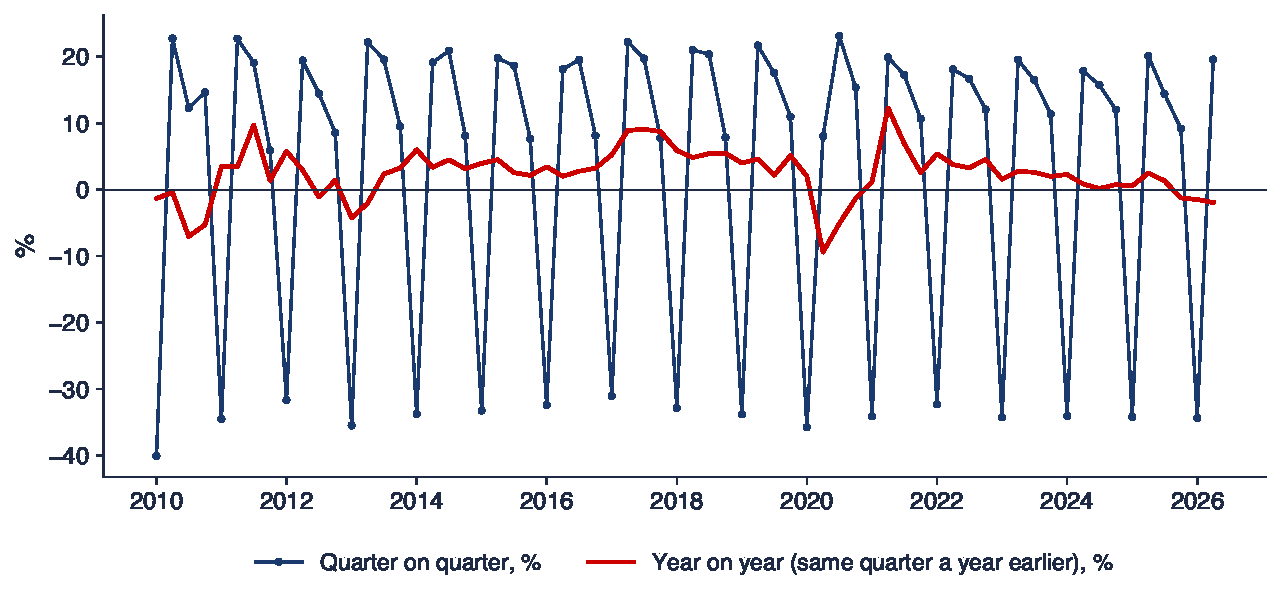
\includegraphics[width=0.94\textwidth,height=0.5\textheight,keepaspectratio]{ch0_sem_b1_growth.pdf}
\end{center}
\vspace{-2mm}
\begin{itemize}
    \item Albastru: rata față de trimestrul anterior oscilează în fiecare an între aproximativ $-35\%$ și $+20\%$; roșu: rata față de anul anterior se mișcă lent, odată cu ciclul economic
    \item \textbf{Interpretare}: doar rata față de anul anterior arată recesiunile (2009--2010, 2020) și încetinirea din 2025--2026; pentru datele neajustate, raportați creșterea față de anul anterior
\end{itemize}
\quantlet{TSA\_ch0\_seminar}{\qlurl{TSA_ch0_seminar}}
\end{frame}

\begin{frame}{B2 [Rezolvat]: EUR/RON: memoria nivelurilor și a variațiilor --- cerință}
\itemsize{\footnotesize}
\begin{itemize}
\item \textbf{Întrebarea}: ajută cursul de azi la prognoza cursului de mîine? Dar variația de azi la prognoza variației de mîine?
\item \textbf{Date}: cursul de referință EUR/RON al BNR, 5 ianuarie 2015 -- 18 septembrie 2026 (2\,939 de zile)
\item \textbf{Cerințe}
\begin{enumerate}
    \item Calculați randamentele logaritmice zilnice $r_t = 100\,(\ln P_t - \ln P_{t-1})$.
    \item Calculați ACF de selecție a nivelului și a randamentelor pentru decalajele 1--20.
    \item Comparați $r_1$ al randamentelor cu banda $\pm 1{,}96/\sqrt T$ și numărați decalajele din afara benzii.
    \item Interpretare: este prognoza naivă un reper potrivit pentru cursul de schimb?
\end{enumerate}
\item \textbf{Raportați}: $r_1$ și $r_{20}$ ale nivelului, $r_1$ și $r_2$ ale randamentelor, banda, numărul decalajelor din afara ei și răspunsul la întrebarea de interpretare
\item Notebook: secțiunea B2
\end{itemize}
\end{frame}

\begin{frame}{B2 [Rezolvat]: Rezolvare (1/2) --- pas cu pas}
\itemsize{\footnotesize}
\begin{itemize}
    \item \textbf{Nivelul}: $r_1 = $ 1{,}00, $r_{20} = $ 0{,}97
    \begin{itemize}
        \item nivelul își amintește valorile pe parcursul a mai multe săptămîni: o descreștere lentă, semnătura unui trend
    \end{itemize}
    \item \textbf{Randamentele}: abaterea standard 0{,}13\% pe zi; $r_1 = $ 0{,}078, $r_2 = $ -0{,}0003
    \begin{itemize}
        \item banda $\pm$0{,}036; 8 din cele 20 de decalaje se află în afara ei
        \item $r_1$ este semnificativ, dar mic: variația de ieri explică mai puțin de 1\% din varianța variației de azi ($r_1^2$)
    \end{itemize}
\end{itemize}
\quantlet{TSA\_ch0\_seminar}{\qlurl{TSA_ch0_seminar}}
\end{frame}

\begin{frame}{B2 [Rezolvat]: Rezolvare (2/2) --- grafic și interpretare}
\itemsize{\footnotesize}
\begin{center}
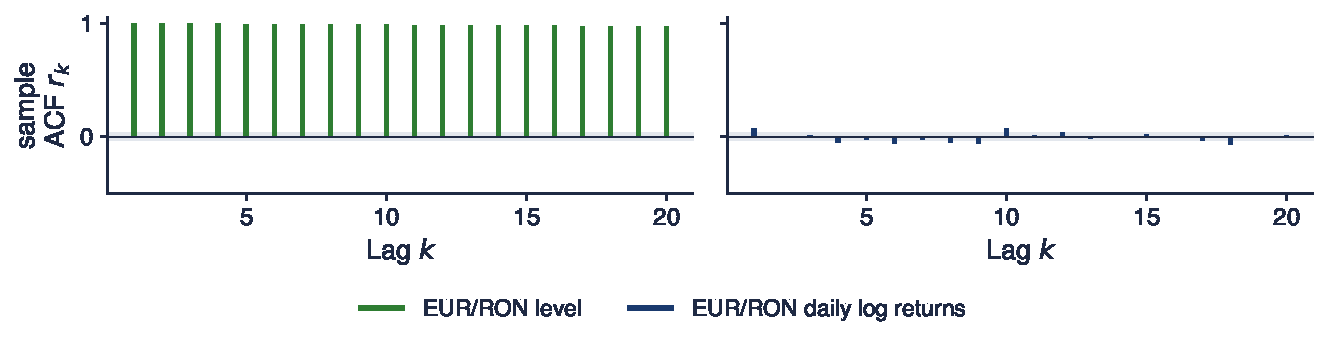
\includegraphics[width=0.94\textwidth,height=0.46\textheight,keepaspectratio]{ch0_sem_b2_acf.pdf}
\end{center}
\vspace{-2mm}
\begin{itemize}
    \item Stînga: ACF a nivelului rămîne aproape de 1; dreapta: ACF a randamentelor este aproape plată; zona colorată: banda $\pm 1{,}96/\sqrt T$
    \item \textbf{Interpretare}: da; nivelul de azi este cea mai bună prognoză simplă a nivelului de mîine, iar variațiile trecute adaugă foarte puțin: prognoza naivă este reperul de depășit
\end{itemize}
\quantlet{TSA\_ch0\_seminar}{\qlurl{TSA_ch0_seminar}}
\end{frame}


%=============================================================================
\section{Rîndul dumneavoastră}
%=============================================================================

\begin{frame}{A4 [Propus]: Alte cifre --- cerință}
\itemsize{\footnotesize}
\begin{itemize}
\item \textbf{Întrebarea}: puteți repeta A1--A3 fără rezolvarea în față?
\item \textbf{Date}: o serie trimestrială 120, 150, 132, 168, 126 (T1 din anul 1 -- T1 din anul 2); o serie 5, 7, 6, 8, 9; o serie cu $m = 3$: antrenare 20, 30, 25, 22, 32, 27, test 23, 33, 29
\item \textbf{Cerințe}
\begin{enumerate}
    \item Model: A1, A2 și A3 [Rezolvat].
    \item Calculați ratele de creștere față de perioada anterioară, diferențele logaritmilor și rata față de anul anterior a ultimului trimestru.
    \item Calculați $r_1$ pentru seria 5, 7, 6, 8, 9 și banda $\pm 1{,}96/\sqrt T$.
    \item Calculați MAE și RMSE ale prognozelor naive și naive sezoniere pentru valorile de test.
\end{enumerate}
\item \textbf{Raportați}: tabelul ratelor de creștere, $r_1$ și banda, cele patru măsuri ale erorii și o propoziție care numește prognoza mai bună
\item Notebook: secțiunea A4
\end{itemize}
\end{frame}

\ifsolutions
\begin{frame}{A4: Rezolvare (profesor)}
\itemsize{\footnotesize}
\begin{itemize}
    \item \textbf{Creștere}
    \begin{itemize}
        \item față de perioada anterioară, \%: $+$25{,}0; -12{,}0, $+$27{,}3; -25{,}0; diferențele logaritmilor: $+$22{,}3; -12{,}8, $+$24{,}1; -28{,}8
        \item față de anul anterior (T1 din anul 2): $100\,(126/120 - 1) = +$5{,}0\%
    \end{itemize}
    \item \textbf{Autocorelația}: $\bar y = 7$, $\sum d^2 = 10$, $\sum d_t d_{t-1} = 1$
    \begin{itemize}
        \item $r_1 = $ 0{,}10; banda $\pm$0{,}88: nu se deosebește de 0
    \end{itemize}
    \item \textbf{Prognoze} (naivă: 27, 27, 27; naivă sezonieră: 22, 32, 27)
    \begin{itemize}
        \item naivă: MAE 4{,}00, RMSE 4{,}32; naivă sezonieră: MAE 1{,}33, RMSE 1{,}41; cîștigă prognoza naivă sezonieră
    \end{itemize}
\end{itemize}
\end{frame}
\fi

\begin{frame}{B3 [Propus]: Inflația din România --- cerință}
\itemsize{\footnotesize}
\begin{itemize}
\item \textbf{Întrebarea}: are inflația lunară un tipar sezonier pe care rata anuală îl ascunde?
\item \textbf{Date}: IAPC al României, 2015 = 100, lunar, 1 ianuarie 2015 -- 1 august 2026 (Eurostat)
\item \textbf{Cerințe}
\begin{enumerate}
    \item Model: B1 și B2 [Rezolvat].
    \item Calculați rata lunară și rata anuală a inflației, în \%.
    \item Calculați inflația lunară medie pentru fiecare lună calendaristică.
    \item Calculați ACF a ratei lunare pentru decalajele 1--24 și pe cea a ratei anuale la decalajul 1.
    \item Interpretare: de ce este rata anuală atît de persistentă?
\end{enumerate}
\item \textbf{Raportați}: ultimele rate lunară și anuală, lunile cu media cea mai mare și cea mai mică, $r_1$ și $r_{12}$ ale ratei lunare, $r_1$ al ratei anuale și răspunsul la întrebarea de interpretare
\item Notebook: secțiunea B3
\end{itemize}
\end{frame}

\ifsolutions
\begin{frame}{B3: Rezolvare (profesor)}
\itemsize{\footnotesize}
\begin{columns}[T]
\begin{column}{0.5\textwidth}
\begin{center}
\includegraphics[width=0.94\textwidth,height=0.42\textheight,keepaspectratio]{ch0_sem_b3_acf.pdf}
\end{center}
\vspace{-2mm}

\end{column}
\begin{column}{0.47\textwidth}
\begin{itemize}
    \item august 2026: lunar $+$0{,}3\%, anual 6{,}3\%; vîrful ratei anuale: 14{,}6\%, în noiembrie 2022
    \item luna cu media cea mai mare: octombrie (0{,}7\%); cea mai mică: iunie (-0{,}1\%)
    \item rata lunară: $r_1 = $ 0{,}48, $r_{12} = $ 0{,}29 (banda $\pm$0{,}17): memorie și un vîrf sezonier
    \item rata anuală: $r_1 = $ 0{,}98: două rate anuale consecutive au în comun 11 din cele 12 variații lunare (ca în sumele mobile ale lui Slutsky)
\end{itemize}
\end{column}
\end{columns}
\end{frame}
\fi

\begin{frame}{B4 [Propus]: Electricitatea: naivă sau naivă sezonieră? --- cerință}
\itemsize{\footnotesize}
\begin{itemize}
\item \textbf{Întrebarea}: pentru producția lunară de electricitate, este prognoza naivă sezonieră mai bună decît cea naivă?
\item \textbf{Date}: producția netă de electricitate a României, TWh pe lună (Eurostat); setul de test: august 2024 -- iulie 2026 (24 de luni)
\item \textbf{Cerințe}
\begin{enumerate}
    \item Model: A3 [Rezolvat].
    \item Împărțiți seria în timp: ultimele 24 de luni formează setul de test.
    \item Prognozați setul de test cu metoda naivă și cu metoda naivă sezonieră ($m = 12$), folosind doar setul de antrenare.
    \item Calculați MAE și RMSE pentru fiecare metodă și reprezentați grafic ambele prognoze, alături de datele de test.
    \item Interpretare: de ce metoda naivă sezonieră nu cîștigă clar aici?
\end{enumerate}
\item \textbf{Raportați}: cele patru măsuri ale erorii, graficul și răspunsul la întrebarea de interpretare
\item Notebook: secțiunea B4
\end{itemize}
\end{frame}

\ifsolutions
\begin{frame}{B4: Rezolvare (profesor)}
\itemsize{\footnotesize}
\begin{columns}[T]
\begin{column}{0.5\textwidth}
\begin{center}
\includegraphics[width=0.94\textwidth,height=0.42\textheight,keepaspectratio]{ch0_sem_b4_forecast.pdf}
\end{center}
\vspace{-2mm}

\end{column}
\begin{column}{0.47\textwidth}
\begin{itemize}
    \item naivă (toate prognozele 3{,}97 TWh): MAE 0{,}28, RMSE 0{,}33
    \item naivă sezonieră: MAE 0{,}28, RMSE 0{,}38
    \item cele două sînt aproape egale: metoda naivă sezonieră copiază iarna puternică din anul de antrenare peste o perioadă de test cu nivel mai scăzut, deci erorile ei de iarnă sînt mari
    \item o metodă care combină sezonalitatea și nivelul (Holt--Winters, la curs) se descurcă mai bine
\end{itemize}
\end{column}
\end{columns}
\end{frame}
\fi


%=============================================================================
\section{Partea C: întrebări deschise}
%=============================================================================

\begin{frame}{C1: O idee de proiect}
\itemsize{\small}
\begin{itemize}
    \item \textbf{Întrebarea}: cît din variația unei serii lunare românești este sezonieră și se schimbă tiparul sezonier în timp?
    \item \textbf{Serii posibile} (Eurostat sau INS)
    \begin{itemize}
        \item producția de electricitate, sosirile de turiști, comerțul cu amănuntul, producția industrială
    \end{itemize}
    \item \textbf{Pași}
    \begin{itemize}
        \item reprezentați grafic seria și creșterea ei față de anul anterior
        \item comparați media fiecărei luni calendaristice în primii și în ultimii cinci ani
        \item după curs: descompuneți seria cu STL și comparați amplitudinea sezonieră în timp
    \end{itemize}
    \item Un prim pas bun pentru proiectul de echipă, legat de \tsachlink{https://danpele.github.io/Time-Series-Analysis/RO/Cursuri/capitol0_introducere.pdf}{Capitolele 0} și \tsachlink{https://danpele.github.io/Time-Series-Analysis/RO/Cursuri/capitol4_sezonalitate_prognoza.pdf}{4}
\end{itemize}
\end{frame}

\begin{frame}[fragile]{C2 [Propus]: Critica unui răspuns generat de AI --- răspunsul}
\itemsize{\footnotesize}
\begin{itemize}
    \item \textbf{Cererea} trimisă unui asistent AI: „Din PIB-ul real trimestrial al României, calculează rata medie anuală de creștere și RMSE pentru o prognoză naivă.”
\end{itemize}
\begin{lstlisting}
g = read_eurostat('namq_10_gdp', 'Q.CLV10_MEUR.NSA.B1GQ.RO') / 1000
growth = g.diff()                                # annual growth rate, %
print('average annual growth:', growth.mean())
test = g.sample(frac=0.2, random_state=1).sort_index()   # test set
train = g.drop(test.index)                               # training set
fc = train.reindex(g.index).ffill().shift(1).reindex(test.index)  # naive
rmse = ((test - fc) ** 2).mean()
print('RMSE of the naive forecast:', rmse)
\end{lstlisting}
\begin{itemize}
    \item \textbf{Concluzia AI}: „PIB-ul României crește cu doar 0{,}24\% pe an, iar prognoza naivă are un RMSE de 111{,}9 miliarde EUR, mai mare decît PIB-ul însuși: prognoza PIB este fără speranță.”
\end{itemize}
\end{frame}

\begin{frame}{C2 [Propus]: Critica unui răspuns generat de AI --- cerință}
\itemsize{\small}
\begin{itemize}
\item \textbf{Întrebarea}: puteți avea încredere într-un cod care rulează fără niciun mesaj de eroare?
\item \textbf{Date}: codul și concluzia de pe slide-ul anterior; definițiile din noțiunile necesare
\item \textbf{Cerințe}
\begin{enumerate}
    \item Model: A1, A3 și B1 [Rezolvat].
    \item Găsiți cele trei greșeli introduse intenționat în cod.
    \item Pentru fiecare greșeală, precizați cum ați detecta-o: o verificare a rezultatului, noțiunile necesare sau un exercițiu rezolvat.
    \item Scrieți codul corectat, cu ultimele 8 trimestre ca set de test, și raportați rezultatele corectate.
    \item Precizați dacă mai rămîne valabilă concluzia „prognoza PIB este fără speranță”.
\end{enumerate}
\item \textbf{Raportați}: cîte o linie pentru fiecare greșeală, în formatul: cerere, răspuns, greșeală, cum a fost găsită, corectare; creșterea și RMSE corectate
\item Notebook: secțiunea C2
\end{itemize}
\end{frame}

\ifsolutions
\begin{frame}{C2: Rezolvare (profesor)}
\itemsize{\footnotesize}
\begin{itemize}
    \item \textbf{Greșeala 1}: \texttt{g.diff()} este o variație în miliarde EUR pe un trimestru, nu o rată anuală de creștere în \%
    \begin{itemize}
        \item detectare: unitățile de măsură (A1, B1); corectare: \texttt{100 * (g / g.shift(4) - 1)}, media 2{,}9\% pe an
    \end{itemize}
    \item \textbf{Greșeala 2}: un set de test aleator; trimestrele de test mai vechi sînt prognozate cu date ulterioare
    \begin{itemize}
        \item detectare: noțiunile necesare (împărțire în timp); corectare: \texttt{train, test = g.iloc[:-8], g.iloc[-8:]}
    \end{itemize}
    \item \textbf{Greșeala 3}: eroarea pătratică medie fără rădăcina pătrată, în (miliarde EUR)$^2$
    \begin{itemize}
        \item detectare: un RMSE mai mare decît seria însăși (A3); corectare: \texttt{np.sqrt(...)}
    \end{itemize}
    \item Corectat, ultimele 8 trimestre: RMSE 8{,}36 miliarde EUR (naivă), 0{,}56 (naivă sezonieră): concluzia nu se susține; un reper sezonier prognozează PIB-ul cu o eroare de aproximativ 1\%
\end{itemize}
\end{frame}
\fi


%=============================================================================
\section{Încheiere}
%=============================================================================

\begin{frame}{Exerciții pentru acasă}
\itemsize{\small}
\begin{itemize}
    \item \textbf{Terminați exercițiile propuse}: A4, B3, B4 și C2
    \begin{itemize}
        \item fiecare indică exercițiul rezolvat care servește drept model
    \end{itemize}
    \item \textbf{Încercați încă o serie}
    \begin{itemize}
        \item repetați B1 pentru PIB-ul zonei euro (cheia \texttt{Q.CLV10\_MEUR.NSA.B1GQ.EA20}) și comparați oscilațiile sezoniere cu cele ale României
    \end{itemize}
    \item \textbf{Rezolvați quiz-ul \tsachlink{https://danpele.github.io/Time-Series-Analysis/RO/Cursuri/capitol0_introducere.pdf}{Capitolului 0}} pe site-ul cursului: 20 de întrebări, cu explicație pentru fiecare răspuns
\end{itemize}
\end{frame}

\begin{frame}{Recapitulare; urmează cursul din \tsachlinkt{https://danpele.github.io/Time-Series-Analysis/RO/Cursuri/capitol0_introducere.pdf}{Capitolul 0}}
\itemsize{\footnotesize}
\begin{columns}[T]
\begin{column}{0.52\textwidth}
\begin{itemize}
    \item \textbf{Azi}
    \begin{itemize}
        \item pentru datele neajustate, raportați creșterea pe un an, nu pe un trimestru
        \item $r_k$: cît își amintește o serie valoarea de acum $k$ perioade
        \item nivelurile cu trend au memorie lungă; variațiile zilnice ale prețurilor au memorie redusă
        \item prognozele naivă și naivă sezonieră sînt reperele; împărțiți în timp, apoi măsurați MAE și RMSE
        \item codul generat de AI poate rula și totuși să fie greșit
    \end{itemize}
\end{itemize}
\end{column}
\begin{column}{0.45\textwidth}
\begin{itemize}
    \item \textbf{La curs}
    \begin{itemize}
        \item Cum este organizat și evaluat cursul?
        \item Ce componente alcătuiesc o serie de timp?
        \item Cum prognozează netezirea exponențială?
        \item Ce prognoze cîștigă pe datele reale ale României?
    \end{itemize}
    \item Seminarul are rol de exercițiu și nu se notează; rezolvările cerințelor [Propus] se discută la seminar
\end{itemize}
\end{column}
\end{columns}
\end{frame}

\end{document}
